\section{Applikation im Dark Mode}

Zu guter Letzt sehen wir uns noch die Applikation im Dark Mode an. Diese Funktionalität ist meiner Meinung nach bei fast allen Webanwendungen ein Muss und genau aus diesem Grund wird sie logischerweise auch bei unserer Webapplikation unterstützt. Dank Angular in Kombination mit Angular Material ist die Umsetzung eines dunklen Modus wirklich nicht schwierig und zieht sich konsistent durch das gesamte Design durch. Dabei ist natürlich wichtig, dass die \emph{Corporate Identity} von Siemens nicht verloren geht, weshalb die Hauptfarbe wieder das ikonische Türkis ist. In den folgenden Abbildungen \ref{fig:AngularDashboardPrototypeDark}, \ref{fig:AngularFindingsPrototypeDark} und \ref{fig:AngularGraphPrototypeDark} können Sie Ihre Blicke über den angenehm zu erblickenden Dark Mode ruhen lassen.

\begin{figure}
    \centering
    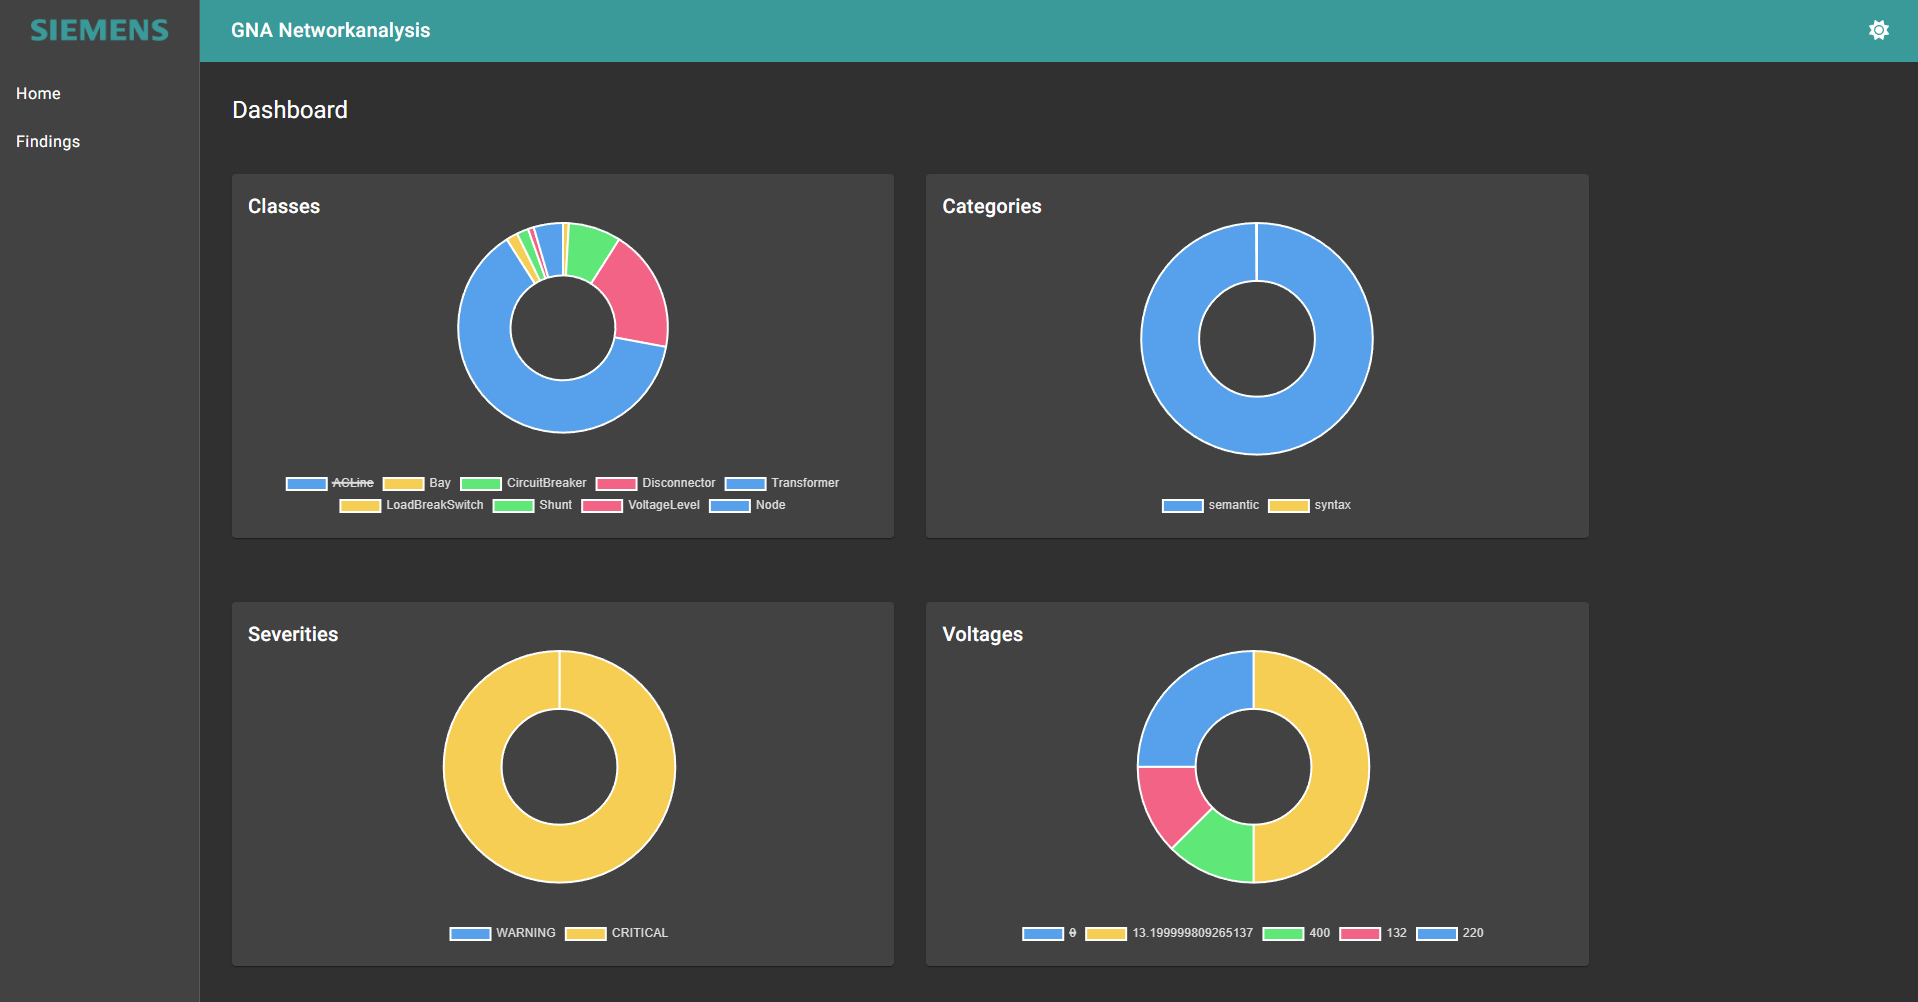
\includegraphics[width=1\textwidth]{content/img/Empire/Frontend/Angular_Dashboard_Prototype_Dark.png}
    \caption{Dashboard im Dark Mode}
    \label{fig:AngularDashboardPrototypeDark}
\end{figure}
\FloatBarrier

\begin{figure}
    \centering
    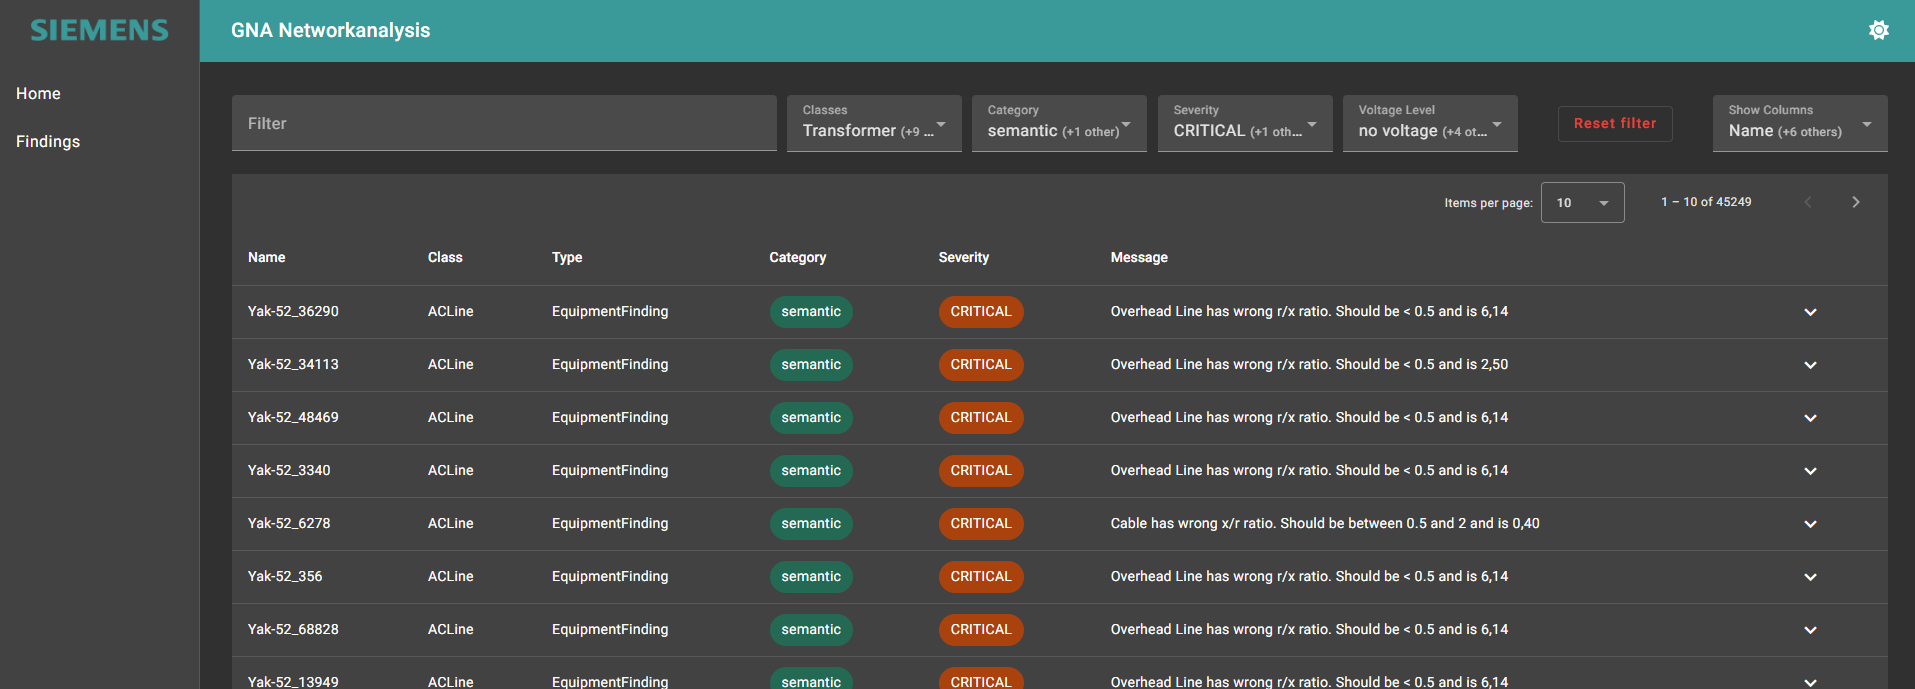
\includegraphics[width=1\textwidth]{content/img/Empire/Frontend/Angular_Findings_Prototype_Dark.png}
    \caption{Ergebnisse des Netzmodells im Dark Mode}
    \label{fig:AngularFindingsPrototypeDark}
\end{figure}
\FloatBarrier

\begin{figure}
    \centering
    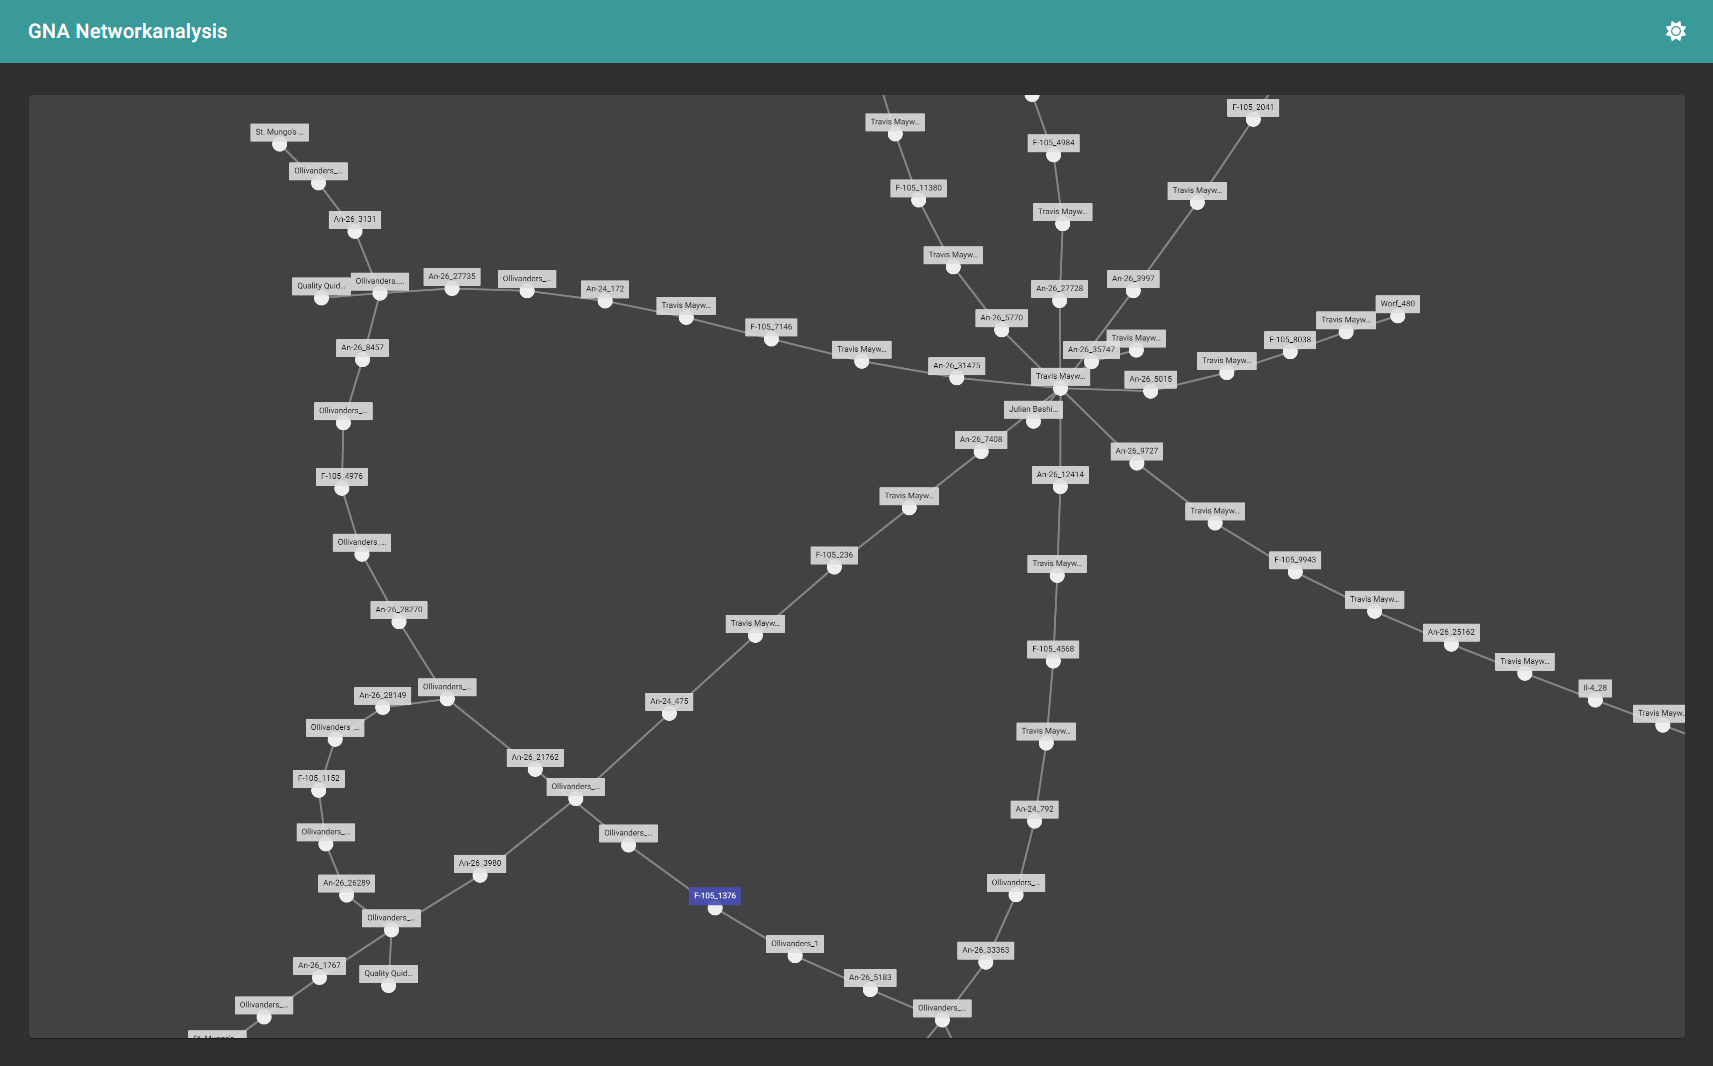
\includegraphics[width=1\textwidth]{content/img/Empire/Frontend/Angular_Graph_Prototype_Dark.png}
    \caption{Visualisierung des Stromnetzmodells mittels Graph im Dark Mode}
    \label{fig:AngularGraphPrototypeDark}
\end{figure}
\FloatBarrier